\documentclass[docid=2017]{comp_test1}
\begin{document}
\setcounter{chapter}{2017}
\exam{2017 Test 1}

\examgroup{First, Follow Sets and Parsers LL(k)}

Consider the CFG (Context-Free Grammar) below.

\begin{enumerate}[wide, noitemsep]
    \item \texttt{S → A T}
    \item \texttt{A → a A a | b A b | \# T}
    \item \texttt{T → a T | b T | $\varepsilon$}
\end{enumerate}

\question
Give the \textit{First} and \textit{Follow} sets for each grammar variable;

\ansseparator

\vspace{-2.0em}
\begin{alignat*}{5}
    & First (S) &&= \{ \texttt{a}, \texttt{b}, \texttt{\#} \} && ~~~~~~~~~~ && Follow(S) &&= \{ \$                         \} \\
    & First (A) &&= \{ \texttt{a}, \texttt{b}, \texttt{\#} \} && ~~~~~~~~~~ && Follow(A) &&= \{ \texttt{a}, \texttt{b}, \$ \} \\
    & First (T) &&= \{ \texttt{a}, \texttt{b}, \varepsilon \} && ~~~~~~~~~~ && Follow(T) &&= \{ \texttt{a}, \texttt{b}, \$ \} \\
\end{alignat*}
\vspace{-3.0em}

\question
Show the table for the parser LL(1);

\ansseparator

\begin{center}
    \small
    \begin{tabular}{@{} c | p{33mm} | p{33mm} | p{33mm} | p{33mm} @{}}
        \multirow{2}{*}{NT} & \multicolumn{4}{c}{T} \\ \cline{2-5}
        & \texttt{a} & \texttt{b} & \texttt{\#} & \$ \\ \hline
        $S$ & 1 & 1 & 1 &  \\ \hline
        $A$ & 2.1 & 2.2 & 2.3 &  \\ \hline
        $T$ & 3.1, 3.3 & 3.2, 3.3 &   & 3.3
    \end{tabular}
\end{center}

\question
Indicate the possible problems this grammar may have and that need to be solved in order it can be implemented as a top-down recursive parser LL(1).

\ansseparator

\noindent
This grammar is not LL(1), which means there is a problem with this grammar being implemented as a top-down recursive LL(1) parser. It is not LL(1) because there is at least one cell with more than one production; this means that, for instance, upon performing a lookahead of 1 to try and decide which production of $T$ to use, if it finds \texttt{a} it still has two possible distinct productions (3.1 and 3.3).

\examgroup{Lexical and Syntactic Analysis}
We intend to design and implement a programming language. The presented CFG G1 below represents the current version of the grammar for the language.

~

\noindent
\begin{minipage}[t]{0.44\textwidth}
    Some of the Tokens for G1:
    
    \begin{itemize}[wide, noitemsep, label={}]
        \small
        \item \texttt{IDENTIFIER = [a-zA-Z][0-9a-zA-Z]*}
        \item \texttt{WHILE = while}
        \item \texttt{ENDWHILE = endwhile}
        \item \texttt{DO = do}
        \item \texttt{IF = if}
        \item \texttt{ELSE = else}
        \item \texttt{THEN=then}
        \item \texttt{ENDIF = endif}
    \end{itemize}
\end{minipage}
\begin{minipage}[t]{0.58\textwidth}
    Grammar G1:
    
    \begin{enumerate}[wide, noitemsep]
        \small
        \item \texttt{S → (Stmt)*}
        \item \texttt{Stmt → While | Assign | If}
        \item \texttt{While → WHILE Cond DO (Stmt)* ENDWHILE}
        \item \texttt{Assign → IDENTIFIER = Operand(OP Operand)?;}
        \item \texttt{Operand → IDENTIFIER | CONST}
        \item \texttt{If → IF Cond THEN Stmt (ELSE Stmt)? ENDIF}
        \item \texttt{Cond → Operand CMP Operand}
    \end{enumerate}
\end{minipage}

\question
Considering that \texttt{OP} represents the arithmetic operations, -, +, *, /,and \texttt{CMP} the comparison operations, $!=$, $==$, $>$, $<$, $>=$, $<=$, show the definitions of these tokens as regular expressions.

\clearpage

\ansseparator

\begin{itemize}[wide, noitemsep, label={}]
    \item \texttt{OP = - | + | * | /}
    \item \texttt{CMP = != | == | < | > | >= | <=}
\end{itemize}

\question
Show the DFA for the tokens WHILE, ENDWHILE, IF, ELSE, and ENDIF.

\ansseparator

\begin{center}
    \small
    \begin{tikzpicture}[->,>=stealth',node distance=4.0em, initial text=$ $,]
        \node[state, initial                    ] (s0)  {$s_0$};
        \node[state,            right of=s0     ] (s6)  {$s_6$};
        \node[state,            above of=s6     ] (s1)  {$s_1$};
        \node[state,            right of=s1     ] (s2)  {$s_2$};
        \node[state,            right of=s2     ] (s3)  {$s_3$};
        \node[state,            right of=s3     ] (s4)  {$s_4$};
        \node[state, accepting, right of=s4     ] (s5)  {$s_5$};
        \node[state, accepting, right of=s6     ] (s7)  {$s_7$};
        \node[state,            below of=s6     ] (s8)  {$s_8$};
        \node[state,            right of=s8     ] (s9)  {$s_9$};
        \node[state,            right of=s9     ] (s10) {$s_{10}$};
        \node[state,            right of=s10    ] (s11) {$s_{11}$};
        \node[state,            below of=s9     ] (s12) {$s_{12}$};
        \node[state,            right of=s12    ] (s13) {$s_{13}$};
        \node[state,            right of=s13    ] (s14) {$s_{14}$};
        \node[state,            right of=s14    ] (s15) {$s_{15}$};
        \node[state,            below of=s14    ] (s16) {$s_{16}$};
        \node[state,            right of=s16    ] (s17) {$s_{17}$};
        \node[state,            right of=s17    ] (s18) {$s_{18}$};
        \node[state,            right of=s18    ] (s19) {$s_{19}$};
        \node[state,            right of=s19    ] (s20) {$s_{20}$};
        
        \draw	   
            (s0)    edge[above] node{w} (s1)
            (s1)    edge[above] node{h} (s2)
            (s2)    edge[above] node{i} (s3)
            (s3)    edge[above] node{l} (s4)
            (s4)    edge[above] node{e} (s5)
            (s0)    edge[above] node{i} (s6)
            (s6)    edge[above] node{f} (s7)
            (s0)    edge[above] node{e} (s8)
            (s8)    edge[above] node{l} (s9)
            (s9)    edge[above] node{s} (s10)
            (s10)   edge[above] node{e} (s11)
            (s8)    edge[above] node{n} (s12)
            (s12)   edge[above] node{d} (s13)
            (s13)   edge[above] node{i} (s14)
            (s14)   edge[above] node{f} (s15)
            (s13)   edge[above] node{w} (s16)
            (s16)   edge[above] node{h} (s17)
            (s17)   edge[above] node{i} (s18)
            (s18)   edge[above] node{l} (s19)
            (s19)   edge[above] node{e} (s20)
        ;

    \end{tikzpicture}
\end{center}

\question
Show the CSTs for the code example below and considering the depicted CFG.

\ansseparator

\vspace{-1em}
\begin{center}
    \ttfamily\small
    \begin{tikzpicture}
        \Tree	[.S
                    [.Stmt
                        [.Assign
                            [.IDENTIFIER
                                A
                            ]
                            =
                            [.Operand
                                [.CONST
                                    3
                                ]
                            ]
                            ;
                        ]
                    ]
                    {Stmt...}
                ]
    \end{tikzpicture}
\end{center}

% \vspace{-2em}
\begin{center}
    \ttfamily\small
    \begin{tikzpicture}
        \Tree	[.Stmt
                    [.While
                        [.WHILE
                            while
                        ]
                        [.Cond
                            [.Operand
                                [.IDENTIFIER
                                    A
                                ]
                            ]
                            [.CMP
                                $>=$
                            ]
                            [.Operand
                                [.CONST
                                    0
                                ]
                            ]
                        ]
                        DO
                        [.Stmt
                            [.Assign
                                [.IDENTIFIER
                                    A
                                ]
                                =
                                [.Operand
                                    [.IDENTIFIER
                                        A
                                    ]
                                ]
                                [.OP
                                    -
                                ]
                                [.Operand
                                    [.CONST
                                        1
                                    ]
                                ]
                            ]
                        ]
                        [.ENDWHILE
                            endwhile
                        ]
                    ]
                ]
    \end{tikzpicture}
\end{center}

\question
Show a possible abstract syntax tree (AST) for the concrete syntax tree of the previous question.

\ansseparator

\vspace{-1em}
\begin{center}
    \ttfamily\small
    \begin{tikzpicture}
        \Tree	[.Stmts
                    [.=
                        A
                        3
                    ]
                    [.While
                        [.$>=$
                            A
                            0
                        ]
                        [.Stmts
                            [.=
                                A
                                [.-
                                    A
                                    1
                                ]
                            ]
                        ]
                    ]
                ]
    \end{tikzpicture}
\end{center}

\question
Show the necessary functions, considering the grammar rules of lines 2 to 3, and the respective pseudo-code to implement them, as a top-down recursive LL(1) parser. Assume the existence of the lexical analyzer which outputs the sequence of tokens, the existence the global variable \textit{token}, and the function \textit{next()} which returns the next token in the sequence of tokens (in the beginning the variable \textit{token} identifies the first token in the sequence).

\ansseparator

\begin{lstlisting}
Stmt(){
    if(token == WHILE) return While();
    if(token == IF   ) return If();
    return Assign();
}

While(){
    if(token != WHILE) return false;
    token = next();
    if(!Cond()) return false;
    if(token != DO) return false;
    token = next();
    while(token != ENDWHILE) if(!Stmt()) return false;
    token = next();
    return true;
}
\end{lstlisting}

\question
Suppose we want to modify the grammar in order to make possible to input values from the keyboard and print values of variable to the screen. Present the grammar modifications you suggest.

\ansseparator

\begin{itemize}[wide, noitemsep]
    \item \texttt{READ = read}
    \item \texttt{WRITE = write}
\end{itemize}

\begin{itemize}[wide, noitemsep]
    \item \texttt{Stmt → While | Assign | If | Read | Write}
    \item \texttt{Read → READ IDENTIFIER;}
    \item \texttt{Write → WRITE IDENTIFIER;}
\end{itemize}

\examgroup{Semantic Analysis}

Consider the segment of Java code of the example below.

\begin{lstlisting}[language=java]
public int f1(int B[]){
    int[] A = {1, 2, 3, 4};
    int S = 0;
    int i;
    for (i = 0; i < A.length; i++) {
        S += A[i]*B[i];
    }
    return S;
}
\end{lstlisting}

\question
Assuming that the variables used in the code can only be parameters or local variables, show a possible symbol table for this example indicating the information to be included in the descriptors.

\ansseparator

\begin{center}
    \begin{tikzpicture}[every node/.style={align=center},level distance=7em]
        \Tree	[.{
                    Functions \\[0.5em]
                    \begin{tabular}{| c |}
                        \hline
                        ... \\ \hline
                        f1 (access: public) \\ \hline
                        ... \\ \hline
                    \end{tabular}
                }
                    {
                        Return \\
                        int
                        \vspace{1.9em}
                    }
                    {
                        Params \\[0.5em]
                        \begin{tabular}{| l |}
                            \hline
                            B (type: int[]) \\ \hline
                        \end{tabular}
                        \vspace{0.9em}
                    }
                    {
                        Locals \\[0.5em]
                        \begin{tabular}{| l |}
                            \hline
                            A (type: int[]; size: 4) \\ \hline
                            S (type: int) \\ \hline
                            i (type: int) \\ \hline
                        \end{tabular}
                    }
                ]
    \end{tikzpicture}
\end{center}

\question

Show a high-level intermediate representation for the example, using as reference the high-level intermediate representation based on expression trees and presented in the classes of the course.

\ansseparator

\vspace{-1em}
\begin{center}
    \ttfamily\small
    \begin{tikzpicture}
        \Tree	[.function
                    [.stl A
                        [.newArray
                            int
                            4
                        ]
                    ]
                    [.sta
                        {ldl A}
                        0
                        1
                    ]
                    [.sta
                        {ldl A}
                        1
                        2
                    ]
                    [.sta
                        {ldl A}
                        2
                        3
                    ]
                    [.sta
                        {ldl A}
                        3
                        4
                    ]
                    [.stl S
                        0
                    ]
                    {for...}
                ]
    \end{tikzpicture}
\end{center}

\begin{center}
    \ttfamily\small
    \begin{tikzpicture}
        \Tree	[.for
                    [.{stl i}
                        0
                    ]
                    [.$<$
                        {ldl i}
                        [.ldf
                            A
                            length
                        ]
                    ]
                    [.{stl S}
                        [.+
                            {ldl S}
                            [.*
                                [.lda
                                    {ldl A}
                                    {ldl i}
                                ]
                                [.lda
                                    {ldp B}
                                    {ldl i}
                                ]
                            ]
                        ]
                    ]
                ]
    \end{tikzpicture}
\end{center}

\question
In some programming languages, such as Java, the indexing of arrays neither can have negative values nor values greater than N-1 (with N the size of the specific array dimension being indexed). Discuss the inclusion of this kind of verification in the semantic analysis of a compiler, mentioning the possible problems and solutions.

\ansseparator

\noindent
This verification implies the semantic analyser knows all the possible values for each variable that can be an index (i.e., integers and longs) by analyzing the assignments made to them. There are two major limitations: (1) the first is that the value of an index may depend on user input, and as such is only known at runtime; (2) the value of an index may result from such complex calculations that its value cannot be known from a simple semantic analysis.

The solutions are: (1) assume initially that it can take all values, and use restrictions (like conditions, for instance) to limit the range of possible values, and if the range of the variable has a value that would otherwise be an invalid index the compiler can warn the user (but should not fail to compile, as the user might wish it should itself be careful with the input); (2) even though those computations might be very complex, they can still be made on compile time, thus the semantic analyser might want to actually run that code in compile time to get the value.

\examgroup{General}

Comment the following sentences, indicating if they are true or false, and justifying your answers (if helpful include illustrative examples to help on justifying your answers):

\question
The existence of ambiguity in a given CFG always implies conflicts in its LL(1) parser table.

\ansseparator

\noindent
True. Ambiguity is equivalent to stating there is a given string $s$ that has more than one valid syntactic tree according to that CGF. This means that, at some point, the parser will have two possible choices, and as such that the parser table has at least one cell with more than one possible production (aka a conflict).

\question
Compilers split the lexical, syntactic and semantic analysis in separated stages because it is impossible to implement them in a single stage.

\ansseparator

False. All stages could be merged into syntactic analysis, as lexical analysis can also be done with CGFs instead of the traditional solution with REs (since a CGF is more powerful than a RE), and semantic analysis can be performed while doing syntactic analysis.

Compilers usually split analysis into those three phases because it makes compilers easier to implement and easier to understand, as well as more efficient; besides, it uses a macroscopic structure that is related to the theoretical analysis of the language, where we apply increasingly complex requirements to the universal language until it becomes the language we want.

\end{document}
